\section{Results}
\label{sec:results}


\subsection{Benchmarks and comparison with existing casters}

The algorithms developed during the internship were finally tested on a few larger scenes which come closer to real world applications of Enlight. The cylinder head used throughout this thesis, cf. for example Figure \ref{fig:cylinder_head}, is often used for quick demonstration or debugging, as it is a rather small scene which can be loaded in roughly a second. Besides the cylinder head, a lot of other scenes, more or less fitting the purpose of Enlight, are available and can be loaded within the main application. From these scenes, two more have been chosen which show interesting behavior. The first additional scene is a Menger sponge, which is a fractal geometry. It is easily created using a programming language. Due to its recursive nature, Menger sponges provide an easy way of generating complex meshes just by adjusting a parameter of the generation script. In the following benchmarks a level five member sponge will be used. The last additional scene for ray casting will be a multi impeller, which is a technical component of many centrifugal pumps. Figure \ref{fig:Menger_sponge_multi_impeller} shows screen shots of the addition scenes.

\begin{figure}
\centering
\includegraphics[width=0.49\textwidth]{Menger_sponge_gl}
\includegraphics[width=0.49\textwidth]{Menger_sponge}
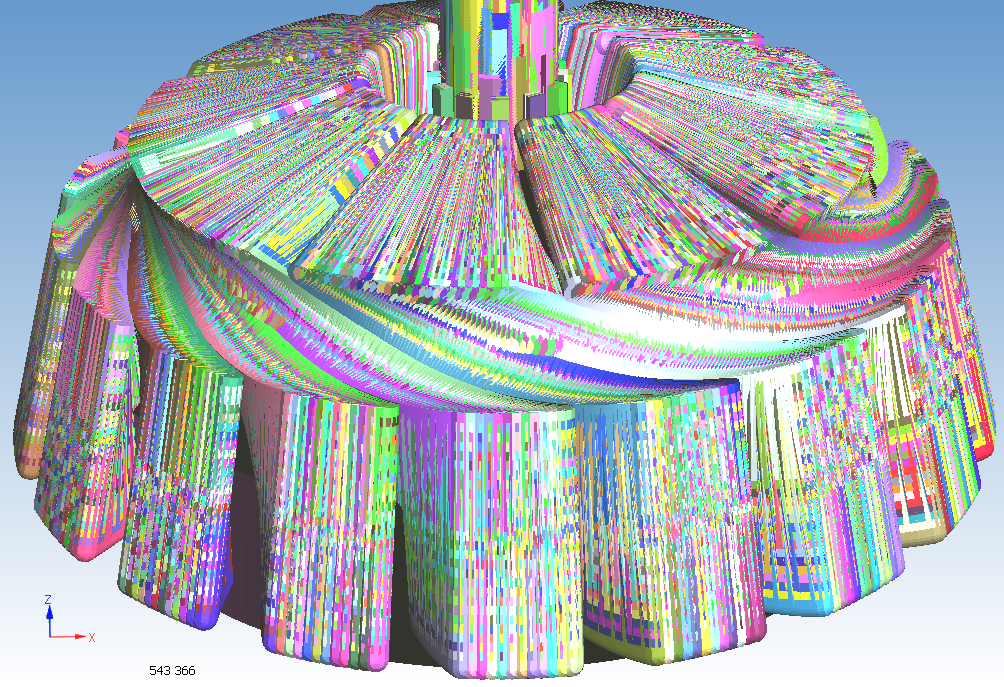
\includegraphics[width=0.49\textwidth]{multi_impeller_gl}
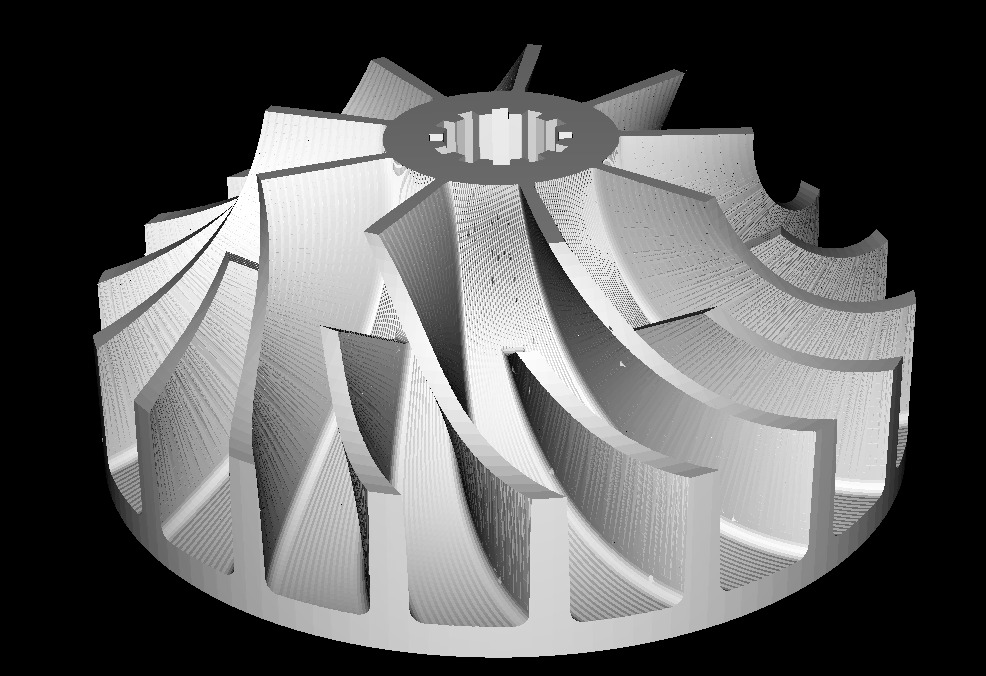
\includegraphics[width=0.49\textwidth]{multi_impeller}
\caption{Screenshots of the OpenGL visualization and the OpenCL kernel output of the SinglePrimaryBooleanCellRayCaster of a level 5 Menger sponge and a multi impeller.}
\label{fig:Menger_sponge_multi_impeller}
\end{figure}

\begin{table}[h]
\centering
\begin{tabular}{|l | r r r r r r r|}
\hline
Scene & Volumes & Unique tri & Cell tri & Grid dim & Outside & Surface & Inside \\
\hline
Cylinder head & 21 & 28000 & 63604 & 40 40 18 & 13392 & 8744 & 6664 \\
Menger sponge 5 & 14044 & 168528 & 9582636 & 100 100 100 & 498480 & 501520 & 0 \\
Multi impeller & 4726 & 12510260 & 4010800 & 150 150 61 & 928405 & 139271 & 304824 \\
\hline
\end{tabular}
\caption{Geometric information about the used test scenes.}
\label{tbl:geometrics}
\end{table}

Table \ref{tbl:geometrics} shows various geometric information about the three scenes used for benchmarking. The cylinder head is rather small with only 21 subtraction volumes and 28,000 triangles. The Menger sponge level five has been chosen for its large number of subtraction volumes. A level six Menger sponge was also tested once, which is the first scene to exceed the 100,000 subtraction volume mark with roughly 110,000 cuboids. However, it consumes the full available system memory and forces the operating system to swap. As a consequence, the classification of the scene takes several hours to complete in which the used work station cannot be used for anything else. Therefore, the level 5 variant has been chosen. An interesting behavior can also be observed on the Menger sponge when having a closer look at Table \ref{tbl:geometrics}. Although the initial geometry of the Menger sponge only consists of around 0.17 million triangles, this number multiplies by almost 57 to 9.58 million when the triangles are assigned to the cells they intersect. This is one of the large drawbacks of using a grid as acceleration structure. The final multi impeller provides a real world example of subtractive manufacturing. It mainly impresses by its large triangle count of 12,5 million. Furthermore, the multi impeller profits tremendously by the cell classification as only 11\% of all cells are surface cells. The smaller number of cell triangles when compared with the original, unique ones is explained by the many subtraction volumes which partly stick out of the grid.

Each scene is loaded and then ray casted ten times by each chosen ray casting implementation using an output resolution of $1024 \times 768$ pixels. The average run time is shown in Table \ref{tbl:cast_times}. All times are in milliseconds.

\begin{table}[h]
\centering
\begin{tabular}{|r | r r r r|}
\hline
Caster & Precision & Cylinder head & Menger sponge 5 & Multi impeller \\
\hline

% 26 27 25 24 25 25 25 26 27 27
% 41 40 43 43 40 40 40 40 40 40
% 114 114 114 114 113 113 115 114 114 115
\multirow{2}{*}{SingleBooleanCell} & single & 25.7 & 40.7 & 114 \\

% 72 72 74 72 72 72 72 72 75 72
% 160 161 161 160 159 159 160 160 159 160
% 655 654 653 654 653 654 655 654 652 653
 & double & 72.5 & 159.9 & 653.7 \\

% 26 26 25 26 25 25 26 26 25 26
% 42 42 42 41 41 41 42 42 41 42
% 124 123 123 123 123 123 123 123 124 123
\multirow{2}{*}{SinglePrimaryBooleanCell} & single & 25.6 & 41.6 & 123.2 \\

% 83 82 83 82 85 82 82 82 82 82
% 260 258 259 259 259 258 258 258 258 258
% 959 954 961 958 953 954 951 959 956 952
 & double & 82.5 & 258.5 & 955.7 \\

% 52 71 62 69 70 64 70 73 78 70
% 880 479 679 675 336 447 641 425 1144 1448
% 1212 925 695 817 738 680 1512 824 714 1024
Packet & single & 67.9 & 715.4 & 914.1 \\

% 47 41 42 48 39 46 46 46 46 48
% 183 161 163 162 181 162 173 151 160 162
% 324 321 314 326 313 313 313 322 314 300
CPU AVX & double & 44.9 & 165.8 & 316 \\

\hline

Update time & & 130 & 11071 & 10455 \\

Transfer time & & 4 & 177 & 334 \\
\hline
\end{tabular}
\caption{Run time of several casters, complete update time and memory transfer time on different test scenes. All times are in milliseconds.}
\label{tbl:cast_times}
\end{table}

The first thing one can notice on the benchmark results is that the single precision variant of the final SinglePrimaryBooleanCell caster is faster in all scenarios than the CPU implementation and produces visually equivalent results than the slower CPU variant which runs in double precision. Furthermore, the cylinder head and the level five Menger sponge can both be casted interactively with 39 and 24 frames per second (FPS). The multi impeller is more calculation intensive only achieving around 8 FPS. Nonetheless, these results are very delighting as they prove that scenes of this complexity can still be ray casted in reasonable time. The SingleBooleanCell caster is surprisingly a little bit faster on larger scenes. However, this small advance is compensated by more erroneous pixels. The packet ray caster is far behind all other ray casting approaches which mostly due to the high amount of synchronization points inside the kernel. Furthermore, switching from single to double precision causes a serious performance loss in all tested kernels. Although a run time decrease by a factor of two to three has been expected, as the Kepler architecture has only a third of double precision units than normal cores, the performance drop was even worse on larger scenes. Nevertheless, single precision has proven to deliver good and stable results in most cases. \\
Apart from the casting times, one should also notice the time required for an update of the OpenCL buffers. Although the memory transfer times seem reasonable, the time required for the complete update is enormous. The most time consuming operations during the update is the flattening process and the calculation of the clipped centroids. The latter could be avoided, if the centroids were precalculated when the triangles are added to the grid.

\subsection{Development}

During the internship various software tools have been used for developing OpenCL applications. Some of the experiences made might be of value for future developers and are therefore shared here:

\begin{description}
\item[NVIDIA Visual Profiler] \hfill \\
This separate tool from NVIDIA is hipped with their CUDA SDK and provides a standalone debugger and profiler for GPGPU applications. Although mainly developed for aiding CUDA developers, it should support OpenCL until CUDA SDK version 4.1. However, this version has been tried without success.

\item[NVIDIA Nsight] \hfill \\
Nsight is NVIDIA's second GPGPU debugging and profiling tool and requires a free registered developer account before it can be downloaded. It provides excellent Visual Studio integration and does support OpenCL according to NVIDIA's website. However, Nsight requires the presence of at least two GPUs, where one is used for debugging kernels step by step and the second one for handling the display while the first one is busy. Nsight also allows remote debugging.

\item[Intel SDK for OpenCL Applications] \hfill \\
Intel also supports OpenCL for their CPUs and on chip graphic controllers. By installing Intel's SDK for OpenCL Applications, one can install additional Visual Studio plugins which allow to create dedicated OpenCL projects. Syntax highlighting for OpenCL source files is configured and a kernel file can be compiled offline using a new context menu entry to check for compilation errors without having to start the actual application. Furthermore, a simple debugger is integrated which allows to debug a single work item which has to be configured before the main application is started. However, this debugger is limited to OpenCL programs on the CPU and cannot be used in the case of crashes as other work items are processed in parallel to the debugging session of the selected one. Also break points do not work when set in files included by a kernel. 
Visual Studio integration, does only run on Intel CPUs, does only allow debugging of one preselected work item. In general, the tool makes a still immature expression although being useful.

\item[gDEBugger] \hfill \\
Graphic Remedy's gDEBugger is a standalone debugger, profiler and memory analyzer for OpenGL and OpenCL applications. It is additionally independent of the used hardware platform and freely available. The tool shows basic information for a process it is attached to like memory consumption of various objects inside open OpenGL or OpenCL contexts. It also offers a time line showing enqueued OpenCL operations like enqueued kernels or memory transfers and highlights their start time and duration. This allows a developer to optimize a devices occupancy. Although the possibility of creating break points at certain API calls and viewing the source code of kernel objects, stepping through kernel code is not supported.

\item[AMD CodeXL] \hfill \\
CodeXL is the name of AMD's flagship in OpenCL development and comes with excellent Visual Studio integration. The tool suite provides a sophisticated debugger which allows debugging all work items in parallel. Therefore, special multi-watch windows can be opened for tracking variables across all work items, shown in a tabular view. Breakpoints and stepping are fully supported within Visual Studio. Furthermore, an application can be launched in profiling mode where CodeXL reads important performance counters from the GPU for each executed kernel. This information is very useful in hunting down bottlenecks and optimizing kernels for specific GPUs. Additionally, a static kernel analyzer is provided which can show the disassembly of a kernel and provides general static information such as consumed registers or required local memory. Unfortunately, CodeXL is limited to AMD cards only and has therefore not been used during the internship. However, it proved to be highly useful during the development of the algorithms presented in the first part of this thesis "GPGPU Computing with OpenCL"
\end{description}

\subsection{Existing problems}

Although the developed ray casters achieve good performance and provide visually satisfying results, there is still room for improvement. One of the biggest problems for the boolean counting kernels is the intersection buffer which requires 1.2 KiB of memory for each work item. This (relatively) large amount of memory cannot be held in registers and is spilled into the slow global memory. Some time was actually spent during the internship on thinking how this buffer could be avoided. A possible alternative is to organize the triangles inside a cell in an intelligent data structure which allows to iterated the triangles depth-sorted, e.g. a BSP tree. However, this would add additional overhead to the grid management routines as these data structures have to maintained or rebuilt each time geometry is added to the grid. Furthermore, data structures also add more complexity to the memory layout of the triangles. Finding a better solution to this problem would probably account for a larger performance boost.

A second problem is the memory access pattern. GPUs are designed for so-called coalesced memory reads, which means that consecutive work items should read from consecutive memory addresses from global memory. This is definitely not the case in all caster implementations, as cells and triangles are accessed at almost random locations. At this point is probably also room for optimization by maybe copying all triangles of a cell  into shared memory using one large fetch across all work items instead of every work item requesting all triangles.

Finally, also the result of a profiler would be very valuable to detect bottlenecks which are not as obvious as the previous ones. However, profiling an OpenCL application on NVIDIA hardware seems to be tedious with the current tools provided by this hardware vendor. Unfortunately, no AMD graphic cards are available at RISC.
